\section{Stetigähnliche Regler \skript{71}}
Bei stetigähnlichen Reglern wird u immer noch auf wenige Werte beschränkt. Mit folgenden Konzepten wird aber erreicht, dass die Strecke trotzdem mehr oder weniger 'stetig' beeinflusst werden kann.
\subsection{Interne Rückkopplung des Reglers (hier mit Zweipunktregler) \skript{71}}
		\begin{minipage}{9cm}
		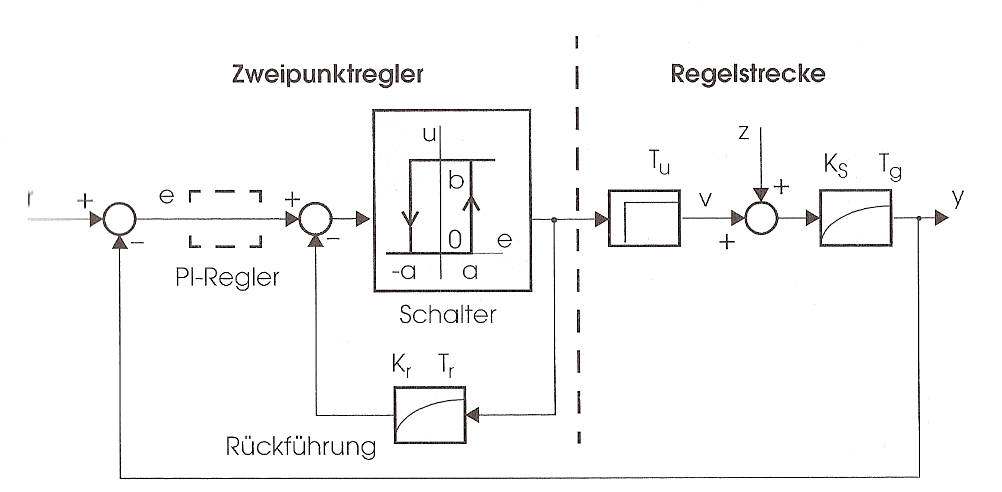
\includegraphics[width=8.5cm]{./bilder/ZweipunktreglerMitRueckfuehrung.jpg}
        \end{minipage}
		\begin{minipage}{7.5cm}
        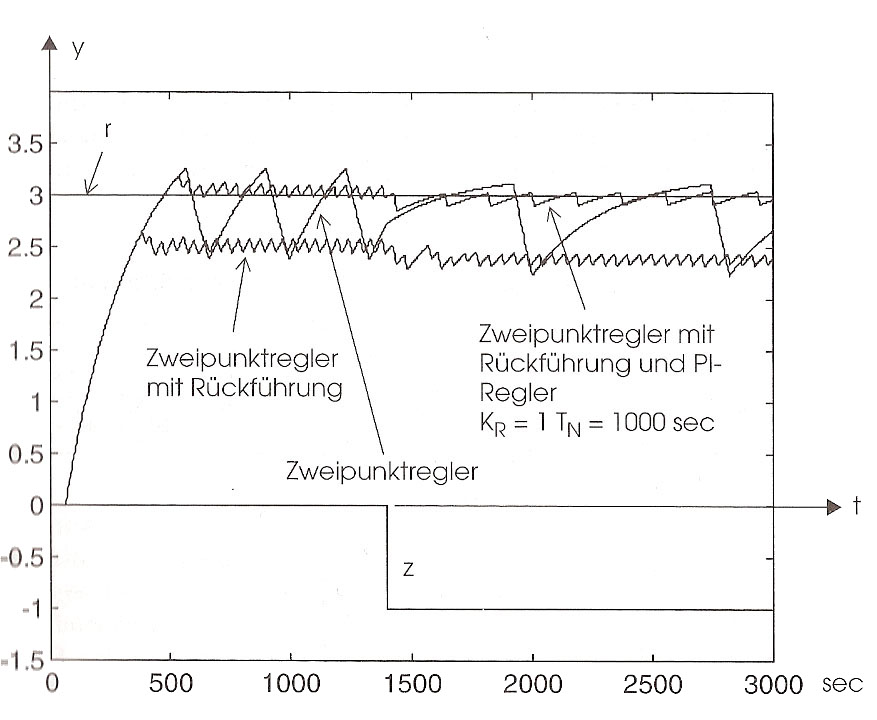
\includegraphics[width=7cm]{./bilder/ZweipunktreglerMitRueckfuehrung_dia.jpg}
        \end{minipage}\\
		Die Rückkopplung mit einem $PT_1$-Glied über dem Zweipunkteregler bewirkt
		einen bedeutend kleineren Rippel. Leider ist der Mittelwert noch unterhalb des
		Sollwertes. Mithilfe eines PI-Reglers vor dem Zweipunkteregler, kann der IST-Wert
		angehoben werden.
\subsection{Regler mit Stellantrieb, Schrittregler (hier mit Dreipunktregler) \skript{73}}	
\begin{minipage}{9cm}
		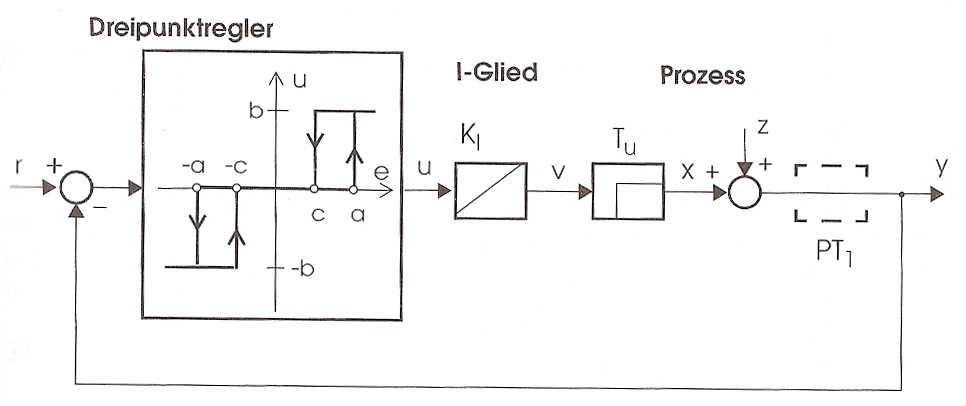
\includegraphics[width=9cm]{./bilder/Dreipunktregler.jpg}
        \end{minipage}
		\begin{minipage}{7.5cm}
        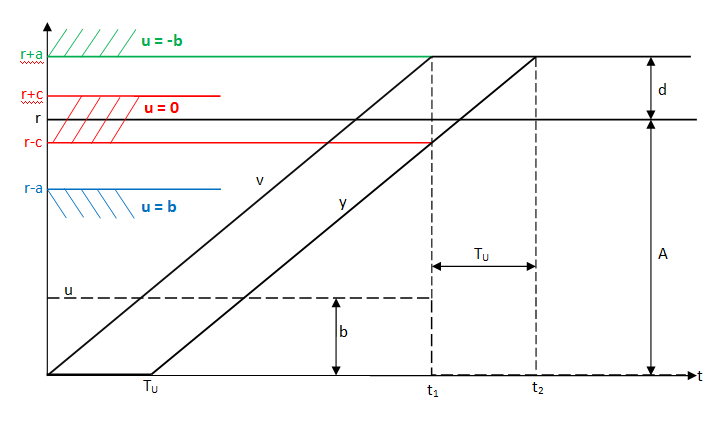
\includegraphics[width=7.5cm]{./bilder/Dreipunktregler_dia.png}
        \end{minipage}\\
		gewünscht: $d = 0 \rightarrow c = K_I \cdot T_u \cdot b$\\
		Falls mit PT$_1$-Glied $\rightarrow c = K_I \cdot K_s \cdot b (T_u + T_G)$
		\newpage